% Compile with XeLaTeX (Overleaf: Menu -> Compiler -> XeLaTeX). Bibliography: BibTeX with IEEEtran.bst.
\documentclass[conference]{IEEEtran}
\usepackage{fontspec}
\setmainfont{texgyretermes}[Extension=.otf, UprightFont=*-regular, BoldFont=*-bold, ItalicFont=*-italic, BoldItalicFont=*-bolditalic]
\newfontfamily\tamilfont[Path=./fonts/, Extension=.ttf, UprightFont=NotoSansTamil-Regular, BoldFont=NotoSansTamil-Bold, Script=Tamil, Scale=0.86]{NotoSansTamil}
\usepackage[Latin,Tamil]{ucharclasses}
\setTransitionsFor{Tamil}{\begingroup\tamilfont}{\endgroup}
\newcommand{\ta}[1]{#1}
\newcommand{\rupee}{{\tamilfont ₹}}
\usepackage{amsmath}
\usepackage{graphicx}
\usepackage{booktabs}
\usepackage{tabularx}
\usepackage{multirow}
\usepackage{array}
\usepackage{xcolor}
\usepackage{tikz}
\usetikzlibrary{positioning,arrows.meta,fit}
\usepackage{cite}
\usepackage[hyphens]{xurl}
\usepackage[colorlinks=true,linkcolor=blue!50!black,citecolor=blue!50!black,urlcolor=blue!60!black]{hyperref}
\definecolor{tblue}{HTML}{2a78d6}
\definecolor{tgray}{HTML}{52514e}
\newcommand{\best}[1]{\textbf{#1}}
\newcommand{\grade}[1]{\textsuperscript{\scriptsize[#1]}}
\renewcommand{\arraystretch}{1.08}
\setlength{\tabcolsep}{3.2pt}
% float placement: allow large top floats so tables stay near their text
\renewcommand{\topfraction}{0.92}\renewcommand{\dbltopfraction}{0.92}
\renewcommand{\textfraction}{0.06}\renewcommand{\floatpagefraction}{0.85}\renewcommand{\dblfloatpagefraction}{0.85}
\setcounter{topnumber}{3}\setcounter{dbltopnumber}{3}\setcounter{totalnumber}{6}

\newcommand{\repo}{\url{https://github.com/Kiranrossi/local-voice-research}}
\newcommand{\colab}[1]{\href{https://colab.research.google.com/github/Kiranrossi/local-voice-research/blob/main/notebooks/#1}{\nolinkurl{#1}}}

\begin{document}

\title{Local Speech Models for English and Tamlish:\\ An Evidence-Based Comparison and a Fine-Tuning Plan for Tamil--English Code-Mixed Speech}

\author{\IEEEauthorblockN{Kiran Guruv S M}
\IEEEauthorblockA{Research assignment submission, October 2026\\
Code, notebooks and raw outputs: \repo}}

\maketitle

\begin{abstract}
We evaluate open-weight speech-to-text (STT) and text-to-speech (TTS) models that run entirely on local hardware, first for English and then for Tamlish (Tamil and English mixed within a sentence). Rather than relying on public leaderboards alone, we built a reproducible harness and measured 7 STT and 4 TTS models on three hardware profiles: an NVIDIA T4 GPU, an 8\,GB Apple M2 laptop GPU, and the same laptop's CPU only. Tests target an Indian deployment: Indian-accented English (Svarah), the author's own recordings containing rupee amounts, phone numbers and Indian names, no-speech clips that expose hallucination, and 30 native-speaker Tamlish recordings plus 30 IndicVoices Tamil clips. Three findings shape the recommendations. (i) Leaderboard rank does not transfer: the leaderboard leader, Qwen3-ASR, corrupted rupee amounts and hallucinated ``okay'' on every silent clip, while Whisper large-v3-turbo was the most accurate on Indian English (7.4\% WER on Svarah, 85\% entity accuracy). (ii) Hardware changes speed, not accuracy: Whisper's WER was identical on GPU, Apple GPU and CPU, but its latency ranged from 0.36\,s to 7.0\,s, so Parakeet-TDT-0.6B-v2 (0.11\,s on CPU) is the CPU-only choice; a voice-activity detector removed Whisper's hallucinations (10/10 to 0/10) at no accuracy cost. (iii) No open model handles Tamlish end to end: IndicConformer hears it almost perfectly (3.3\% script-agnostic phonetic error) but can only write English words in Tamil script, while Whisper large-v3 writes the target mixed script but transcribes spontaneous Tamil poorly (42.5\%). We therefore propose LoRA fine-tuning of Whisper large-v3 on real and synthetic code-mixed data whose transcripts are converted to a single mixed-script convention, with IndicConformer as a pseudo-labelling teacher, and success criteria set against the measured baselines.
\end{abstract}

\begin{IEEEkeywords}
speech recognition, text-to-speech, on-device inference, code-switching, Tamil, Indian English, benchmarking
\end{IEEEkeywords}

% =====================================================================
\section{Executive Summary}
\label{sec:summary}
We assume a real-time, on-premise voice assistant for Indian users with commercial deployment (Section~\ref{sec:assumptions}). Table~\ref{tab:recs} gives our recommendations; every number is reproducible from the repository~\cite{repo}.

\begin{table}[!t]
\caption{Recommendations (measured unless marked ``est.'')}
\label{tab:recs}
\footnotesize
\begin{tabularx}{\columnwidth}{@{}p{1.55cm}X@{}}
\toprule
\textbf{Setting} & \textbf{Recommendation and reason} \\
\midrule
STT, GPU (T4; RTX 4090 est.) & \best{Whisper large-v3-turbo + Silero VAD}~\cite{mc_whisperturbo,gh_silero}: best Indian-English WER (7.4\%) and entity accuracy (85\%), 0.36\,s/sentence on T4, MIT, supports Tamil. \textit{Fallback:} Parakeet-TDT-0.6B-v2~\cite{mc_parakeet} (0.12\,s, no hallucination, CC-BY-4.0, English only). \\
STT, Apple laptop (8\,GB M2) & \best{Whisper turbo via MLX + VAD}: 5.6\% WER on 50 Svarah clips, 1.2\,s/sentence, 2.1\,GB. \textit{Fallback:} Parakeet v2 on CPU. \\
STT, CPU only & \best{Parakeet-TDT-0.6B-v2, int8 ONNX}: 7.2\% WER, 0.11\,s/sentence, 2.1\,GB. Whisper fails the real-time gate on CPU (6.6--7.0\,s). \textit{Fallback:} Moonshine Streaming medium (9.5\%, 1.3\,s). \\
TTS (all profiles) & \best{Kokoro-82M}~\cite{mc_kokoro}: highest UTMOS (4.50), lowest round-trip WER (7.3\%), 0.94\,s/sentence on the M2 CPU, Apache-2.0. \textit{Fallback:} Chatterbox~\cite{chatterbox} (MIT, voice cloning; RTF 1.09 on T4, $\approx$0.35 est.\ on RTX 4090). \\
Tamlish & No existing open model is adequate. \best{Fine-tune STT first}: LoRA on Whisper large-v3 with mixed-script transcripts; IndicConformer as teacher (Section~\ref{sec:obj2}). TTS second, via text normalisation plus Indic Parler-TTS. \\
\bottomrule
\end{tabularx}
\end{table}

% =====================================================================
\section{Introduction}
Cloud speech APIs send every utterance off-premise and bill per minute. Open-weight models have closed much of the accuracy gap~\cite{srivastav2025openasr,pinggystt,pinggytts}, but three practical questions remain for an Indian product: which models are accurate for Indian speakers, which run fast enough on the hardware actually available, and which licences permit commercial use. For Tamlish, a further question is whether anything works at all.

\textbf{Contributions.} (1) A reproducible harness that runs every model on the same clips with the same normaliser, timing and memory measurement, on four hardware profiles. (2) Indian-context tests that public leaderboards lack: Indian-accented English, entity accuracy for amounts, numbers and names, and hallucination on silence. (3) A zero-shot Tamlish test on native-speaker recordings with a script-agnostic metric, which shows that most ``errors'' are a writing-convention mismatch rather than mishearing. (4) A fine-tuning plan revised against these measurements. (5) A licence audit and a log of deployment problems encountered.

% =====================================================================
\section{Background and Related Work}
\textbf{Open STT.} Whisper~\cite{radford2022whisper} remains the most widely deployed open model; large-v3-turbo prunes its decoder from 32 to 4 layers for speed~\cite{pinggystt}. On the Open ASR Leaderboard~\cite{openasrlb,srivastav2025openasr} (9 Oct.\ 2026 update), Qwen3-ASR-1.7B~\cite{qwen3asr2026} leads open models at 5.40\% average WER, and NVIDIA's Parakeet-TDT~\cite{xu2023tdt} offers near-top accuracy at 6,000$\times$ real time~\cite{pinggystt}. A 2026 study found that 6 of 11 models reproduce errors in benchmark references, so low leaderboard WER partly measures benchmark fitting~\cite{hfbenchopt}. This motivates testing on independent data.

\textbf{Indian English and Indic resources.} Svarah~\cite{javed2023svarah} provides 9.6\,h of Indian-accented English from 117 speakers. AI4Bharat's IndicVoices~\cite{javed2024indicvoices} contains 7,348\,h of mostly spontaneous speech in 22 languages (1,639\,h transcribed at release), IndicVoices-R~\cite{sankar2024indicvoicesr} provides 99\,h of TTS-grade Tamil, and Vistaar~\cite{bhogale2023vistaar} fine-tunes Whisper on 10.7k\,h of Indian-language data. IndicConformer~\cite{mc_indicconformer,gh_indicconformer} covers all 22 scheduled languages but not English.

\textbf{Code-switched ASR.} MUCS 2021~\cite{diwan2021mucs} released Hindi--English and Bengali--English code-switched data. Microsoft's work on Tamil--, Telugu-- and Gujarati--English (177\,h of Tamil--English training data) showed that code-switch training can erode monolingual accuracy unless monolingual data is kept~\cite{shah2020cs,taskagnostic2020}. Recent Whisper adaptations use LLM-generated code-mixed text with synthesised audio~\cite{biswas2025hinglish}, soft prompts~\cite{yang2025spt}, text-first decoder adaptation~\cite{asyncswitch2025}, and phrase-level audio splicing that includes Tamil--English~\cite{seacs2025}. A community Tanglish LoRA reports 0.976$\rightarrow$0.682 WER on a synthetic test set~\cite{mc_tanglishlora}; a Whisper turbo fine-tune for English--Hebrew reports a 63.8\% WER reduction~\cite{hebrish}. A commercial Hinglish model outputs mixed script, with English in Latin and Hindi in Devanagari~\cite{mc_shunya}.

% =====================================================================
\section{Method}
\subsection{Shortlisting}
Inclusion rule: open weights, a licence permitting commercial use, fits one 24\,GB GPU, and either a top-10 open ranking on the Open ASR Leaderboard~\cite{openasrlb} or Speech Arena~\cite{aaspeecharena}, or a distinct strength such as CPU or edge use. Table~\ref{tab:shortlist} lists the candidates.

\textbf{Excluded, with reasons.} STT: Cohere Transcribe (gated, no timestamps, built for long recordings), Voxtral Small 24B ($\approx$55\,GB in bf16), VibeVoice-ASR (8.7B, meeting-oriented), Canary-Qwen-2.5B (English-only, no accuracy gain)~\cite{pinggystt}. TTS: the top two open-weight Speech Arena models, Breeze TTS~2 (Elo 1,215) and Fish Audio S2 Pro (1,125), plus Voxtral TTS (CC BY-NC 4.0), Higgs Audio V3 and XTTS v2 all carry \emph{non-commercial weight licences}, even where the code repository shows Apache-2.0~\cite{pinggytts}. Reading down the leaderboard without checking weight licences would recommend a model the company cannot ship.

\begin{table*}[!t]
\caption{Shortlisted models. Published figures from the Open ASR Leaderboard (9 Oct.\ 2026) and Speech Arena (Aug.\ 2026) via~\cite{pinggystt,pinggytts}; RTFx = audio seconds per compute second (H200), higher is faster.}
\label{tab:shortlist}
\footnotesize
\begin{tabularx}{\textwidth}{@{}p{4.1cm} p{1.25cm} p{1.35cm} p{2.6cm} p{3.6cm} X@{}}
\toprule
\textbf{Model} & \textbf{Size} & \textbf{Licence} & \textbf{Languages} & \textbf{Published evidence} & \textbf{Why shortlisted} \\
\midrule
\multicolumn{6}{@{}l}{\textit{Speech-to-text}}\\
Qwen3-ASR 1.7B / 0.6B~\cite{qwen3asr2026,gh_qwen3asr} & 1.7B / 0.6B & Apache-2.0 & 30 (incl.\ Hindi; no Tamil) & Avg WER 5.40 / 6.24; RTFx 819 & Most accurate open model on the leaderboard \\
Parakeet-TDT-0.6B v2 / v3~\cite{mc_parakeet,xu2023tdt} & 0.6B & CC-BY-4.0 & English / 25 European & 6.02 / 6.18; RTFx 5,988 / 6,132 & Near-top accuracy at about 7$\times$ the speed \\
Whisper large-v3-turbo~\cite{mc_whisperturbo,radford2022whisper} & 809M & MIT & 99 incl.\ Tamil & 7.64; RTFx 794 & Ecosystem standard; base candidate for Tamlish \\
Granite Speech 5.0 TurboCTC~\cite{mc_granite} & 470M & Apache-2.0 & English & 6.38; RTFx 21,174 & Fastest model on the board \\
Moonshine Streaming tiny / medium~\cite{mc_moonshine,jeffries2024moonshine} & 34M / 245M & MIT & English & Tiny: 12.0, RTFx 847 & Built for CPU and edge streaming \\
\midrule
\multicolumn{6}{@{}l}{\textit{Text-to-speech}}\\
Kokoro-82M~\cite{mc_kokoro,li2023styletts2} & 82M & Apache-2.0\textsuperscript{a} & 8 (no Tamil) & Arena Elo 1,060 & Best quality per compute; CPU-capable \\
Chatterbox~\cite{chatterbox} & 0.5B & MIT\textsuperscript{b} & 23 & Elo 1,020 & Best-rounded MIT model; cloning and emotion control \\
Qwen3-TTS 0.6B~\cite{gh_qwen3tts} & 0.6B & Apache-2.0 & 10 & Not ranked & Heavily used; voice design \\
VoxCPM2~\cite{gh_voxcpm} & 2B & Apache-2.0 & 30 & Not ranked; vendor RTF $\approx$0.30 on RTX 4090 & 48\,kHz output, CPU path \\
\bottomrule
\multicolumn{6}{@{}l}{\scriptsize \textsuperscript{a}Inference depends on espeak-ng (GPLv3)~\cite{mc_kokoro}. \textsuperscript{b}Every output carries an inaudible PerTh watermark~\cite{pinggytts}.}
\end{tabularx}
\end{table*}

\subsection{Hardware profiles}
\textbf{NVIDIA GPU:} Google Colab, Tesla T4 (16\,GB, $\approx$320\,GB/s, no native bf16)~\cite{hw_t4}. \textbf{Apple GPU:} MacBook Air M2, 8\,GB unified memory, via MLX. \textbf{CPU only:} the same laptop with GPU paths disabled (4 performance threads). \textbf{RTX 4090:} not available to us; we estimate it from T4 measurements (Section~\ref{sec:4090}). The fanless M2 throttles under sustained load, so runs were short with cool-down breaks.

\subsection{Test sets}
\begin{table}[!t]
\caption{Test sets}
\label{tab:sets}
\footnotesize
\begin{tabularx}{\columnwidth}{@{}p{2.6cm} r X@{}}
\toprule
\textbf{Set} & \textbf{Clips} & \textbf{Purpose} \\
\midrule
LibriSpeech test-clean~\cite{panayotov2015librispeech,ds_esb} & 100 & Sanity check against published WER \\
Svarah~\cite{javed2023svarah,ds_svarah} & 150 (50 on Mac) & Indian-accented English \\
Own English & 10 & Laptop mic; amounts, phone and reference numbers, times, 18 Indian names/places \\
No-speech & 10 & 5 near-silent, 5 noise; hallucination rate \\
Own Tamlish & 30 & Native speaker; 10 light, 10 medium, 10 heavy mixing \\
IndicVoices Tamil~\cite{ds_indicvoices} & 30 & Real spontaneous Tamil (validation split) \\
TTS sentences & 20 & 10 everyday replies + 10 English stress sentences \\
\bottomrule
\end{tabularx}
\end{table}
Random samples use seed 42. All 40 own recordings passed an automatic quality check (speech 28--36\,dB above the noise floor, no clipping, at least 0.5\,s of lead-in silence). They are recorded by one speaker in one room, which we treat as a limitation (Section~\ref{sec:limits}).

\subsection{Metrics}
\label{sec:metrics}
\textbf{STT:} word error rate (WER) after Whisper's English normaliser plus Indian-English formatting rules, applied identically to references and outputs (``\rupee{}'', ``Rs'' and ``rupees'' are equivalent; ``7:45'' and ``745''; ``T N'' and ``TN''). This removed formatting artefacts that had doubled some models' WER on our clips without changing any wrong amount or name into a correct one. We report 95\% bootstrap confidence intervals over utterances, the real-time factor (RTF = processing time $\div$ audio duration), median latency per sentence at batch size 1 after two warm-up clips, peak memory, hallucination rate (share of no-speech clips producing any text), and entity accuracy (26 amounts, numbers, times and names that must appear exactly).

\textbf{TTS:} RTF and latency; round-trip intelligibility (Whisper large-v3-turbo transcribes each generated clip and we compute WER against the input); predicted naturalness with UTMOS~\cite{saeki2022utmos,gh_speechmos}; and a blind listening test (32 loudness-matched clips, ACR 1--5 scale, model names hidden).

\textbf{Tamlish.} Plain WER penalises correct output: ``account'' and \ta{அக்கவுண்ட்} are both right. We therefore report strict WER, mixed error rate (MER; English words as units, Tamil as characters~\cite{diwan2021mucs}), and a \emph{script-agnostic phonetic CER}. For this metric, each word is romanised and reduced to a coarse phonetic key (vowels dropped after the first letter; k/g, p/b/f, t/d and s/ch/sh merged), so ``office'' and \ta{ஆபீஸ்} both map to \texttt{aps}. We also report English-word recall in either script, the \emph{Latin-English rate} (share of English words written in Latin script, our target convention), the wrong-language rate (Tamil reference, mostly Latin output), and runaway outputs (more than twice the reference length plus 5 words). The matcher found 26/26 English loanwords written in Tamil script in a hand-built check. It is lenient on short words that differ only in a vowel; a native-speaker audit (Section~\ref{sec:obj2}) catches such cases.

\subsection{Scoring and evidence grades}
Every claim carries an evidence grade: [A] independent benchmark or peer-reviewed paper, [B] vendor card, [C] blog or community model, [D] our small-sample test. For each hardware profile, STT candidates first pass two hard gates, commercial licence and real time (RTF $<$ 1). They are then scored on accuracy (Svarah WER, 30\%), speed (log latency, 25\%), licence (20\%), Indian/Tamil readiness (own-clip WER and Tamil support, 15\%) and deployability (10\%; 0.5 if a VAD is required). Criteria are min--max scaled, and a sensitivity run sets accuracy to 50\%. Fig.~\ref{fig:pipeline}(a) shows the pipeline.

\begin{figure*}[!t]
\centering
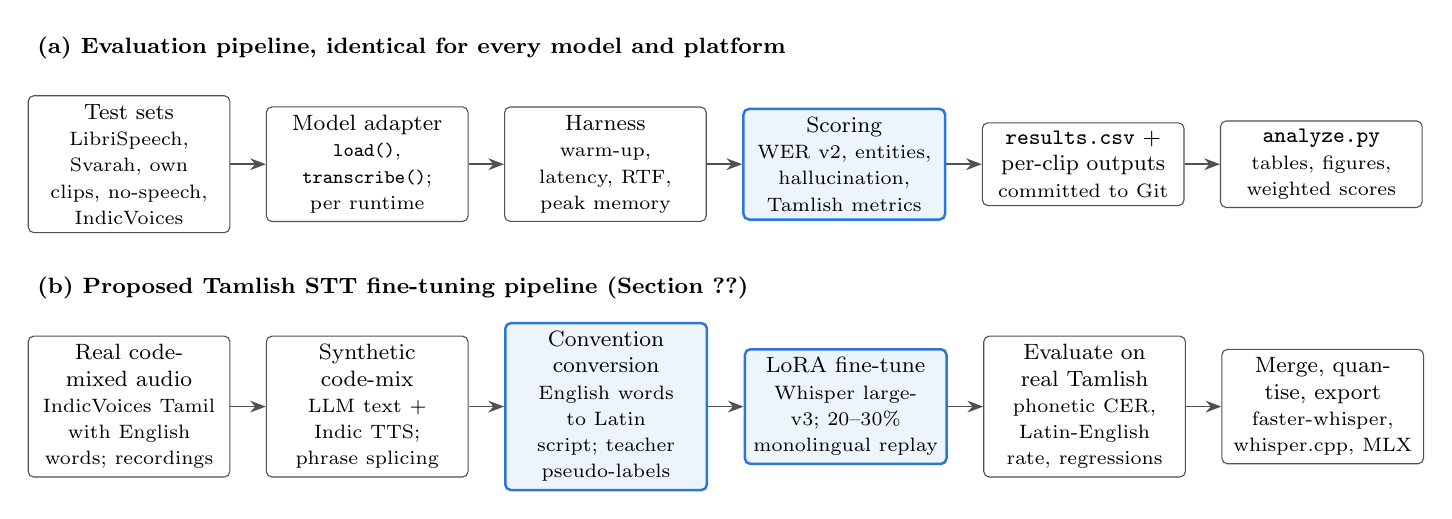
\begin{tikzpicture}[font=\footnotesize, node distance=4mm and 4.5mm,
  box/.style={draw=tgray, rounded corners=2pt, align=center, inner sep=3pt, minimum height=8.5mm, text width=2.35cm, fill=white},
  hl/.style={box, draw=tblue, line width=0.9pt, fill=tblue!8},
  arr/.style={-{Stealth[length=2mm]}, draw=tgray, line width=0.6pt}]
\node[box] (a1) {Test sets\\{\scriptsize LibriSpeech, Svarah, own clips, no-speech, IndicVoices}};
\node[box, right=of a1] (a2) {Model adapter\\{\scriptsize \texttt{load()}, \texttt{transcribe()}; per runtime}};
\node[box, right=of a2] (a3) {Harness\\{\scriptsize warm-up, latency, RTF, peak memory}};
\node[hl, right=of a3] (a4) {Scoring\\{\scriptsize WER v2, entities, hallucination, Tamlish metrics}};
\node[box, right=of a4] (a5) {\texttt{results.csv} + per-clip outputs\\{\scriptsize committed to Git}};
\node[box, right=of a5] (a6) {\texttt{analyze.py}\\{\scriptsize tables, figures, weighted scores}};
\foreach \i/\j in {a1/a2,a2/a3,a3/a4,a4/a5,a5/a6} \draw[arr] (\i) -- (\j);
\node[anchor=west, font=\footnotesize\bfseries] at ([yshift=6mm]a1.north west) {(a) Evaluation pipeline, identical for every model and platform};
\node[box, below=13mm of a1] (b1) {Real code-mixed audio\\{\scriptsize IndicVoices Tamil with English words; recordings}};
\node[box, right=of b1] (b2) {Synthetic code-mix\\{\scriptsize LLM text + Indic TTS; phrase splicing}};
\node[hl, right=of b2] (b3) {Convention conversion\\{\scriptsize English words to Latin script; teacher pseudo-labels}};
\node[hl, right=of b3] (b4) {LoRA fine-tune\\{\scriptsize Whisper large-v3; 20--30\% monolingual replay}};
\node[box, right=of b4] (b5) {Evaluate on real Tamlish\\{\scriptsize phonetic CER, Latin-English rate, regressions}};
\node[box, right=of b5] (b6) {Merge, quantise, export\\{\scriptsize faster-whisper, whisper.cpp, MLX}};
\foreach \i/\j in {b1/b2,b2/b3,b3/b4,b4/b5,b5/b6} \draw[arr] (\i) -- (\j);
\node[anchor=west, font=\footnotesize\bfseries] at ([yshift=6mm]b1.north west) {(b) Proposed Tamlish STT fine-tuning pipeline (Section~\ref{sec:obj2})};
\end{tikzpicture}
\caption{Evaluation and fine-tuning pipelines. Highlighted steps are where this work departs from standard practice: Indian-English and script-agnostic scoring, and converting all transcripts to one mixed-script convention before training.}
\label{fig:pipeline}
\end{figure*}

% =====================================================================
\section{Objective 1: English Results}
\label{sec:obj1}
\subsection{Speech-to-text}
Table~\ref{tab:stt} gives every STT run and Fig.~\ref{fig:stt} plots accuracy against latency. On the T4, our Whisper turbo LibriSpeech WER (1.0\% on 100 clips) is consistent with published values, which validates the harness.

\begin{table*}[!t]
\caption{STT results (scoring v2). Svarah: 150 clips on T4, the first 50 on the Mac. Libri.\ = LibriSpeech test-clean (100 clips). Own = own English clips. Halluc.\ = no-speech clips producing text (of 10). Latency = median per sentence, batch 1.}
\label{tab:stt}
\footnotesize
{\setlength{\tabcolsep}{2.6pt}\begin{tabular*}{\textwidth}{@{\extracolsep{\fill}}l l l r r r r r r r@{}}
\toprule
\textbf{Model} & \textbf{Platform} & \textbf{Runtime / precision} & \textbf{Libri.} & \textbf{Svarah WER [95\% CI]} & \textbf{Own} & \textbf{Entities} & \textbf{Halluc.} & \textbf{Latency} & \textbf{Mem.} \\
\midrule
Whisper large-v3-turbo & T4 & transformers, fp16 & \best{1.0\%} & \best{7.4\%} [5.6, 9.7] & \best{5.8\%} & \best{22/26} & 8 & 0.36\,s & 1.8\,GB \\
Qwen3-ASR 1.7B & T4 & qwen-asr, fp16 & 1.4\% & 8.4\% [6.4, 10.8] & 12.5\% & 18/26 & 10 & 0.86\,s & 4.3\,GB \\
Parakeet-TDT 0.6B v3 & T4 & NeMo, fp32 & 1.6\% & 9.1\% [7.1, 11.4] & 14.4\% & 13/26 & \best{0} & 0.12\,s & 2.8\,GB \\
Parakeet-TDT 0.6B v2 & T4 & NeMo, fp32 & \best{1.0\%} & 9.3\% [7.3, 11.4] & 10.6\% & 18/26 & \best{0} & 0.12\,s & 2.7\,GB \\
Qwen3-ASR 0.6B & T4 & qwen-asr, fp16 & 1.5\% & 9.5\% [7.6, 11.8] & 11.5\% & 20/26 & 10 & 0.85\,s & 1.8\,GB \\
Moonshine Str.\ medium & T4 & transformers, fp16 & 1.4\% & 12.1\% [8.6, 16.7] & 11.5\% & 21/26 & \best{0} & 0.49\,s & 1.4\,GB \\
Moonshine Str.\ tiny & T4 & transformers, fp16 & 3.8\% & 23.4\% [16.6, 34.2] & 29.8\% & 14/26 & \best{0} & 0.24\,s & 0.7\,GB \\
\midrule
Whisper large-v3-turbo & M2 GPU & mlx-whisper, fp16 & -- & 5.6\% [3.5, 8.3] & 5.8\% & 22/26 & 10 & 1.17\,s & 2.1\,GB \\
Parakeet-TDT 0.6B v2 & M2 CoreML+CPU & onnx-asr, int8 & -- & 6.6\% [4.2, 9.8] & 9.6\% & 17/26 & 0 & 0.40\,s & 4.6\,GB \\
\midrule
Whisper turbo + VAD & M2 CPU & faster-whisper, int8 & -- & 5.4\% [3.3, 8.1] & \best{4.8\%} & 22/26 & \best{0} & 6.63\,s & 2.1\,GB \\
Whisper large-v3-turbo & M2 CPU & faster-whisper, int8 & -- & 5.8\% [3.5, 8.8] & 5.8\% & 22/26 & 10 & 6.97\,s & 1.8\,GB \\
Parakeet-TDT 0.6B v2 & M2 CPU & onnx-asr, int8 & -- & 7.2\% [4.5, 10.8] & 11.5\% & 17/26 & 0 & \best{0.11\,s} & 2.1\,GB \\
Moonshine Str.\ medium & M2 CPU & transformers, fp32 & -- & 9.5\% [5.4, 15.8] & 11.5\% & 21/26 & 0 & 1.29\,s & 2.4\,GB \\
\bottomrule
\end{tabular*}}
\end{table*}

\begin{figure}[!t]
\centering
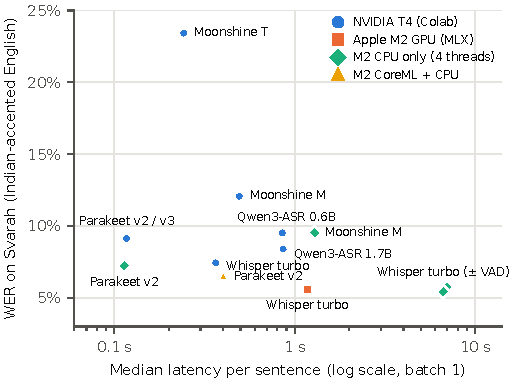
\includegraphics[width=\columnwidth]{figures/stt_accuracy_latency.pdf}
\caption{STT accuracy on Indian-accented English against latency (log scale). Mac points use the first 50 Svarah clips.}
\label{fig:stt}
\end{figure}

\textbf{Finding 1: leaderboard rank does not transfer to Indian use.} Qwen3-ASR leads the leaderboard~\cite{openasrlb} but trails Whisper turbo on Svarah, though the confidence intervals overlap. On our clips it was about twice as error-prone and corrupted amounts: ``\rupee{}2,499'' became ``rupees 200499'' and ``\rupee{}12,350'' became ``1200350''. It also substituted a different real name (Venkataraman to Venkataraghavan). Both Qwen3-ASR sizes produced ``okay'' or ``I am sorry'' on all 10 no-speech clips. Indian proper names were the weakest category for every model: the best got 15/18 names, Parakeet v3 only 5/18. One Svarah clip that every model failed lists festival names from Sikkim and Nepal, not a broken reference [D].

\textbf{Finding 2: a VAD is required for Whisper.} Whisper turbo produced text on 8--10 of 10 no-speech clips on every platform. With faster-whisper's Silero VAD filter~\cite{gh_fasterwhisper,gh_silero}, this fell to 0/10 with no accuracy loss (5.4\% vs 5.8\% on Svarah-50; overlapping intervals), and silent audio was skipped (RTF 0.002). Parakeet and Moonshine never hallucinated.

\textbf{Finding 3: hardware changes speed, not accuracy.} Scored on the same 50 Svarah clips, Whisper turbo reached 5.7\% on the T4 (fp16), 5.6\% on the M2 GPU (MLX) and 5.7\% on the CPU (int8), and identical WER on our clips (5.8\%). int8 quantisation cost nothing measurable. Latency, however, spanned 0.36\,s, 1.17\,s and 6.97\,s. On CPU only, Whisper is too slow for a live assistant (RTF $>$ 1), while Parakeet v2 takes 0.11\,s, about 60$\times$ faster on the same cores. A counter-intuitive result: ONNX Runtime silently selected CoreML on macOS, which split the model across processors and was 3.5$\times$ \emph{slower} (0.40\,s) than forcing the CPU provider.

\textbf{Weighted ranking.} On the T4, the base weights rank Parakeet v2 first (0.86), Parakeet v3 second (0.85) and Whisper turbo third (0.81); with accuracy at 50\%, Whisper ranks first. On the M2 GPU, Whisper (MLX) scores 0.70 against 0.53 for Parakeet (CoreML). On CPU only, Whisper is removed by the real-time gate and Parakeet v2 (0.91) leads Moonshine (0.38). We recommend Whisper turbo + VAD on GPU despite Parakeet's narrow base-score lead, because the score does not capture two decisive requirements: entity accuracy (22/26 vs 18/26) and a Tamil path for Objective~2 (Parakeet is English-only).

\subsection{Text-to-speech}
Table~\ref{tab:tts} and Fig.~\ref{fig:tts} summarise TTS. All four models read the 10 everyday sentences almost perfectly (round-trip WER 0--2.9\%). Errors concentrate in the stress sentences (14--18\%): Indian place names, ``\rupee{}1.5 lakh'' and digit strings. Chatterbox, for example, read ``\rupee{}12,350'' unintelligibly. Kokoro is both the most intelligible and, by UTMOS, the most natural, and it is the only model faster than real time on a CPU (RTF 0.25 on the M2). The single-listener blind test (the author, 8 clips per model) preferred Qwen3-TTS (4.38) and Chatterbox (4.12) over Kokoro (3.62) and VoxCPM2 (3.38). It disagrees with UTMOS and is too small to rank models, so we report it as indicative only [D].

\begin{table}[!t]
\caption{TTS results. RTF on the fastest measured platform; RTX 4090 values are estimates (Section~\ref{sec:4090}).}
\label{tab:tts}
\footnotesize
\begin{tabularx}{\columnwidth}{@{}X r r r r r@{}}
\toprule
\textbf{Model} & \textbf{UTMOS} & \textbf{Listen.} & \textbf{RT-WER} & \textbf{RTF (where)} & \textbf{4090 est.} \\
\midrule
Kokoro-82M & \best{4.50} & 3.62 & \best{7.3\%} & \best{0.25} (M2 CPU) & -- \\
Chatterbox & 4.43 & 4.12 & 9.2\% & 1.09 (T4) & $\approx$0.35 \\
Qwen3-TTS 0.6B & 4.33 & \best{4.38} & 10.1\% & 2.46 (T4, fp32) & $\le$0.79 \\
VoxCPM2 & 3.69 & 3.38 & 8.7\% & 2.00 (T4) & $\approx$0.30\textsuperscript{v} \\
\bottomrule
\multicolumn{6}{@{}p{\columnwidth}@{}}{\scriptsize RT-WER: round-trip WER, all 20 sentences. Listen.: blind test, 1 listener. Peak memory: Kokoro 1.0\,GB (CPU), Chatterbox 3.4, Qwen3-TTS 4.8, VoxCPM2 5.7\,GB. \textsuperscript{v}Vendor-reported~\cite{pinggytts}.}
\end{tabularx}
\end{table}

\begin{figure}[!t]
\centering
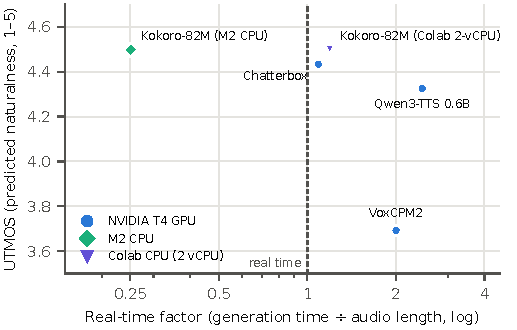
\includegraphics[width=\columnwidth]{figures/tts_quality_speed.pdf}
\caption{TTS predicted naturalness against real-time factor (log). Points left of the dashed line are faster than real time. The same Kokoro model is 4.7$\times$ faster on the M2's four cores than on Colab's two virtual CPUs.}
\label{fig:tts}
\end{figure}

\subsection{RTX 4090 estimates}
\label{sec:4090}
We could not measure an RTX 4090. Batch-1 decoding is mostly memory-bandwidth bound, and the 4090 has about 3.1$\times$ the T4's bandwidth (1,008 vs $\approx$320\,GB/s)~\cite{hw_4090,hw_t4}. We therefore estimate 4090 latency as T4 latency $\div$ 3.1 [D]: Whisper turbo $\approx$0.12\,s, Parakeet $\approx$0.04\,s, Chatterbox RTF $\approx$0.35. Qwen3-TTS and VoxCPM2 should gain more, because the T4 forced fp32 or emulated bf16 (we observed fp16 overflow crashes for Qwen3-TTS and the warning ``T4 does not support bfloat16'' for VoxCPM2). For VoxCPM2 the vendor reports RTF $\approx$0.30~\cite{pinggytts}. All shortlisted models fit in the 4090's 24\,GB. These figures are planning estimates, not measurements.

\subsection{Deployment friction}
Table~\ref{tab:friction} lists the problems we hit. These affect deployability as much as accuracy does.
\begin{table}[!t]
\caption{Deployment problems encountered (Colab, Python 3.13, Oct.\ 2026)}
\label{tab:friction}
\footnotesize
\begin{tabularx}{\columnwidth}{@{}l X@{}}
\toprule
\textbf{Model} & \textbf{Problem $\rightarrow$ resolution} \\
\midrule
Granite 5.0 & Needs a newer \texttt{transformers} than Qwen3-ASR's package pins $\rightarrow$ separate environment; not measured \\
Kokoro & Reference package fails to build (old spaCy on Py 3.13) $\rightarrow$ \texttt{kokoro-onnx}~\cite{gh_kokoroonnx} \\
Qwen3-TTS & fp16 overflow crashes the T4 $\rightarrow$ fp32 \\
Chatterbox & Pins its own PyTorch; torchvision mismatch $\rightarrow$ remove torchvision \\
Moonshine Str. & Input must be a multiple of 80-sample frames $\rightarrow$ zero-pad $\le$20\,ms \\
Whisper-medium (Tamil) & Outdated generation config rejects \texttt{language=} $\rightarrow$ load base config \\
IndicConformer & ONNX Runtime rejects HF-cache symlinks $\rightarrow$ copy real files \\
Parakeet ONNX (Mac) & CoreML auto-selected, 3.5$\times$ slower $\rightarrow$ force CPU provider \\
\bottomrule
\end{tabularx}
\end{table}

% =====================================================================
\section{Objective 2: Tamlish}
\label{sec:obj2}
\subsection{Does any existing model handle Tamlish?}
We tested five setups (Table~\ref{tab:tamlish}, Fig.~\ref{fig:tamlish}): Whisper turbo (Tamil forced, and auto-detect), Whisper large-v3~\cite{mc_whisperv3}, an Apache-2.0 Whisper-medium fine-tuned on Tamil corpora at IIT Madras~\cite{mc_whispertamil}, and IndicConformer-600M. Qwen3-ASR, the leaderboard leader, does not list Tamil~\cite{gh_qwen3asr}.

\begin{table*}[!t]
\caption{Zero-shot Tamlish and Tamil results (T4). Phon.\ CER = script-agnostic phonetic CER. EN recall: English words recognised in either script. Latin-EN: English words written in Latin script (target convention). L/M/H: phonetic CER by mixing level.}
\label{tab:tamlish}
\footnotesize
{\setlength{\tabcolsep}{2.6pt}\begin{tabular*}{\textwidth}{@{\extracolsep{\fill}}l r r r r r c r r r r@{}}
\toprule
& \multicolumn{6}{c}{\textbf{Own Tamlish recordings (30)}} & \multicolumn{3}{c}{\textbf{IndicVoices Tamil (30)}} & \\
\cmidrule(lr){2-7}\cmidrule(lr){8-10}
\textbf{Model} & \textbf{Strict WER} & \textbf{MER} & \textbf{Phon.\ CER} & \textbf{EN recall} & \textbf{Latin-EN} & \textbf{L / M / H} & \textbf{Phon.\ CER} & \textbf{Wrong lang.} & \textbf{Runaway} & \textbf{Latency} \\
\midrule
IndicConformer 600M & 63.9\% & 103.9\% & \best{3.3\%} & \best{95.2\%} & 0\% & 2.3 / 3.7 / 3.5 & \best{7.7\%} & 0\% & 0 & \best{0.18\,s} \\
Whisper large-v3 & \best{46.2\%} & \best{62.0\%} & 5.0\% & 90.4\% & \best{26.9\%} & 7.6 / 2.1 / 5.7 & 42.5\% & 0\% & 0 & 2.05\,s \\
Whisper-medium (Tamil FT) & 64.4\% & 97.5\% & 5.3\% & 86.5\% & 0\% & 2.3 / 2.6 / 8.5 & 22.3\% & 0\% & 0 & 1.68\,s \\
Whisper turbo (ta forced) & 63.9\% & 81.9\% & 10.1\% & 82.7\% & 12.5\% & 4.6 / 14.3 / 9.9 & 82.1\% & 10\% & 5 & 0.51\,s \\
Whisper turbo (auto-detect) & 64.9\% & 83.8\% & 11.8\% & 82.7\% & 12.5\% & 12.2 / 14.3 / 9.9 & 117.3\% & 60\% & 1 & 0.68\,s \\
\bottomrule
\end{tabular*}}
\end{table*}

\begin{figure*}[!t]
\centering
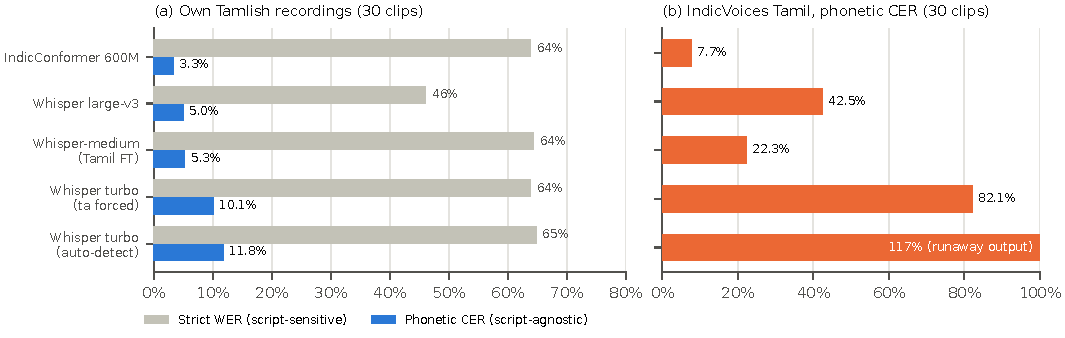
\includegraphics[width=\textwidth]{figures/tamlish_zero_shot.pdf}
\caption{(a) On our Tamlish clips, strict WER ($\approx$64\%) hides near-correct recognition: script-agnostic phonetic CER is 3--12\%. (b) On spontaneous IndicVoices Tamil, the Tamil-specialised models lead and Whisper turbo produces runaway, repetitive output.}
\label{fig:tamlish}
\end{figure*}

\begin{table}[!t]
\caption{Example outputs (own recordings)}
\label{tab:examples}
\footnotesize
\begin{tabularx}{\columnwidth}{@{}l X@{}}
\toprule
\multicolumn{2}{@{}l}{\textbf{ta\_26}\quad \ta{Online payment fail ஆயிடுச்சு, but amount debit ஆயிடுச்சு.}}\\
IndicConf. & \ta{ஆன்லைன் பேமெண்ட் ஃபெயில் ஆயிடுச்சு பட் அமௌண்ட் டெபிட் ஆயிடுச்சு} \\
Large-v3 & \ta{online payment fail ஆயிடுச்சு but amount debit ஆயிடுச்சு} \\
Turbo & \ta{online payment fail ஆயிடித்து but amount debit ஆயிடித்து} \\
\midrule
\multicolumn{2}{@{}l}{\textbf{ta\_11}\quad \ta{என் account-ல balance check பண்ணணும்.}}\\
IndicConf. & \ta{என் அக்கவுண்டில் பேலன்ஸ் செக் பண்ணணும்} \\
Turbo & \ta{ஏன் அக்கும்ட்டல் பாலன்ஸ் செக்கப் பண்ணனும்} \\
Tamil FT & \ta{ஏன் அக்கவுண்ட்ல பேலன்ஸ் செக் பண்ணனும்} \\
\bottomrule
\end{tabularx}
\end{table}

\textbf{Findings.} (1) \emph{Most of the apparent error is a writing-convention mismatch.} All models score $\approx$46--65\% strict WER on our clips but 3.3--11.8\% phonetic CER. IndicConformer recognised 95\% of English words, but always wrote them in Tamil script (Table~\ref{tab:examples}). (2) \emph{The training data shares this convention.} IndicVoices transcripts write English loanwords in Tamil script; our 30-clip sample contained only 2 Latin-script words, although English loanwords such as \ta{ஹெல்ப்} (``help'') were common. A model fine-tuned on such data, like the Tamil Whisper-medium, learns Tamil-script English. (3) \emph{No model combines Tamil hearing with the target format.} Only Whisper large-v3 writes English in Latin script, and only 26.9\% of the time; it is weak on spontaneous Tamil (42.5\%) and normalises colloquial forms (\ta{சொல்லுவாங்க} becomes \ta{சொல்வாங்க}, \ta{அதுக்கு} becomes \ta{அதற்கு}). (4) \emph{Turbo is unsuitable for Tamil}: pruning the decoder costs about 5 points of phonetic CER on Tamlish and causes runaway repetition on 5/30 IndicVoices clips; on auto-detect it switched to English for 60\% of them. (5) A native-speaker audit found one meaning error that the metric under-penalises: turbo and the Tamil Whisper-medium wrote \ta{ஏன்} (``why'') for \ta{என்} (``my''). IndicConformer's outputs on the audited clips were judged fully correct apart from script.

\textbf{Caveats.} IndicConformer was trained by AI4Bharat on IndicVoices, so its IndicVoices lead may partly reflect domain familiarity, even on the validation split. Our Tamlish clips are clean read speech from one speaker, so these numbers are a best case.

\subsection{Which target matters most: STT first}
In a voice assistant, users \emph{speak} Tamlish naturally, and an STT failure breaks the whole pipeline. The assistant's replies, by contrast, can be phrased in cleaner Tamil or English. The STT gap is also larger: no model meets the target convention, while Indian TTS models already speak Tamil, and much of code-mixed TTS can be handled by text normalisation~\cite{gh_hinglishtts}. For the LLM layer between them, open models with Indian-language training already exist (e.g., Sarvam-30B, Apache-2.0), so the gap is in the speech layers.

\subsection{Base model: Whisper large-v3 (evidence-revised)}
Our pre-test plan assumed Whisper turbo. The measurements reversed that choice. We select \textbf{Whisper large-v3 + LoRA} because (i) its tokenizer already writes both scripts, so no vocabulary surgery is needed; (ii) it is the only candidate already emitting Latin-script English, which is the hardest behaviour to teach; (iii) it has the best strict WER and the second-best phonetic CER on Tamlish; (iv) it is MIT-licensed and deployable through faster-whisper, whisper.cpp and MLX~\cite{gh_fasterwhisper,gh_whispercpp,gh_mlxwhisper}. Its weakness, spontaneous Tamil, is exactly what IndicVoices training data provides. The \textbf{alternative base}, decided by a one-hour pilot on the dev set, is the Tamil Whisper-medium (stronger Tamil, smaller). \textbf{IndicConformer is not a base model:} it lacks English tokens, so it would need vocabulary surgery, but it is the best \emph{teacher} for pseudo-labelling untranscribed Tamil audio. If large-v3's latency (2.0\,s on T4, est.\ $\approx$0.65\,s on RTX 4090) is too high for deployment, the fine-tuned model can be distilled into the turbo architecture.

\subsection{Data plan}
\begin{table}[!t]
\caption{Training and evaluation data}
\label{tab:data}
\footnotesize
\begin{tabularx}{\columnwidth}{@{}p{2.45cm} X@{}}
\toprule
\textbf{Source} & \textbf{Use and processing} \\
\midrule
IndicVoices Tamil~\cite{javed2024indicvoices} & Real spontaneous speech with natural English loanwords. Convert transcripts: English loanwords in Tamil script to Latin script \\
Untranscribed IndicVoices audio & Pseudo-label with IndicConformer, then convert as above (teacher--student) \\
Synthetic code-mix & LLM-written Tamlish sentences voiced by Indic Parler-TTS~\cite{mc_indicparler}; phrase splicing of Tamil and Indian-English clips~\cite{seacs2025} \\
Monolingual replay & Tamil and Svarah-style Indian English (20--30\%) to prevent forgetting~\cite{shah2020cs} \\
Real Tamlish recordings & \textbf{Dev/test only}: 3--5\,h from 20+ speakers, mixed-script transcripts; never synthetic \\
\bottomrule
\end{tabularx}
\end{table}
Target: 50--100\,h of training audio, at least 30\% real. \textbf{Convention conversion} (Fig.~\ref{fig:pipeline}b) is the key new step. A loanword lexicon can be mined by aligning IndicConformer's Tamil-script output with Whisper large-v3's Latin-script output on the same audio, using the phonetic keys of Section~\ref{sec:metrics}. An LLM transliteration pass with native-speaker spot checks can cover the remainder. The 30 recorded clips serve as a seed dev set.

\subsection{Approach, compute and success criteria}
\textbf{Approach:} (1) optional text-first adaptation of the decoder on mixed-script Tamlish text~\cite{asyncswitch2025}; (2) LoRA on encoder and decoder attention, with high-switch utterances oversampled $\times$2--3 and monolingual replay mixed in; (3) full fine-tuning only if LoRA plateaus; (4) merge, quantise (int8), then re-run the latency tests of Section~\ref{sec:obj1}.
\textbf{Compute (estimate [D]):} 100\,h $\times$ 3 epochs $\approx$ 36k 30-second windows; at an assumed 1--4 windows/s on one RTX 4090 or A100, this takes $\approx$3--12 GPU-hours, to be confirmed by the pilot.
\textbf{Success criteria}, fixed before training and measured on real Tamlish from unseen speakers:
\begin{itemize}
\item Phonetic CER $\le$ 5\% (zero-shot large-v3: 5.0\% on read speech) and Latin-English rate $\ge$ 90\% (zero-shot best: 26.9\%).
\item IndicVoices Tamil phonetic CER $\le$ 22\%, at least halving large-v3's 42.5\%.
\item No more than +1 point absolute WER on Svarah (English) and on monolingual Tamil, against the base model measured before training.
\item Zero runaway outputs; wrong-language rate $\le$ 2\%; native-speaker meaning-error audit on 100 utterances.
\item Real time on the target hardware after quantisation (RTF $<$ 1 on an M2 via MLX).
\end{itemize}

\subsection{TTS plan (secondary)}
Base: Indic Parler-TTS (Apache-2.0, 0.9B, Tamil and English; gated)~\cite{mc_indicparler,lyth2024parler}. IndicF5~\cite{mc_indicf5,chen2024f5} is an alternative, but its licence tag could not be confirmed as unrestricted, and its card now recommends AI4Bharat's newer Indic-Speak. Step 1 is a text front end: number and currency expansion, and per-word script normalisation so that English words are pronounced as English~\cite{gh_hinglishtts}. Step 2 is fine-tuning on IndicVoices-R Tamil~\cite{sankar2024indicvoicesr} plus code-mixed sentences. Measures: round-trip phonetic CER, a per-word English pronunciation check, and native-speaker MOS on code-mixed sentences.

\subsection{Lessons from Hinglish and other code-mixed work}
(1) Data, not architecture, is the bottleneck; synthetic code-mix from LLM text with TTS, or from audio splicing, consistently helps~\cite{biswas2025hinglish,seacs2025}. (2) Keep monolingual data in the mix to avoid forgetting~\cite{shah2020cs}. (3) Decide the output script convention early: mixed script has worked well for Hinglish~\cite{mc_shunya}, and our results show that the convention of the training data dominates the output. (4) Evaluate on real speech only; the community Tanglish LoRA's synthetic test set~\cite{mc_tanglishlora} cannot show real-world gains.

\textbf{Transfer to Kanglish.} The pipeline transfers to Kannada--English unchanged. IndicVoices, IndicVoices-R and IndicConformer all cover Kannada. Expect less data, so the plan relies more on synthetic code-mix.

% =====================================================================
\section{Limitations: where evidence is thin}
\label{sec:limits}
\begin{itemize}
\item \textbf{Small samples:} 10 own English clips and 30 Tamlish clips from one speaker in one room. Confidence intervals are reported and overlapping intervals are not treated as wins.
\item \textbf{Listening test:} one listener so far; it disagrees with UTMOS and is reported as indicative only.
\item \textbf{RTX 4090:} estimated from bandwidth ratios, not measured. Colab's free GPU quota also forced the Objective-2 tests onto a second account.
\item \textbf{Phonetic metric:} our own design. It is coarse, lenient on vowel-only differences (\ta{ஏன்}/\ta{என்}), and needs a human audit.
\item \textbf{Moonshine} ran through general-purpose \texttt{transformers} rather than its edge runtime, so its CPU speed is probably understated. Granite 5.0 could not be run alongside Qwen3-ASR.
\item \textbf{Thermal throttling:} the fanless M2 may slow under sustained load. \textbf{Leaderboard figures} were taken from dated secondary summaries~\cite{pinggystt,pinggytts} and the live boards move.
\end{itemize}

\section{Assumptions}
\label{sec:assumptions}
(1) The use case is a real-time voice assistant for Indian users, deployed on-premise and commercially. (2) ``Local'' means no network calls at inference, so API-only models (e.g., Sarvam's speech APIs) are out of scope. (3) Non-commercial weight licences are excluded from recommendations. (4) The Tamlish output convention is Tamil words in Tamil script and English words in Latin script. (5) Small-sample results show direction, not statistical proof.

\section{Reproducibility and Artefacts}
Everything is in the public repository~\cite{repo}: raw per-clip outputs for every run, \texttt{results\_scored.csv} files, and \texttt{src/analyze.py} and \texttt{paper/make\_figures.py}, which regenerate every table and figure. Notebooks (open in Colab): \colab{01_stt_colab.ipynb} (English STT), \colab{02_tts_colab.ipynb} (English TTS and scoring), \colab{03_tamlish_colab.ipynb} (Tamlish zero-shot). Mac runners: \texttt{src/run\_mac.py}, \texttt{run\_mac\_tts.py}, \texttt{run\_mac\_tamlish.py}. Scoring: \texttt{src/harness.py} (WER v2, timing, memory), \texttt{tamlish.py} (Tamlish metrics), \texttt{tts\_bench.py}. Tools: \texttt{tools/recorder.html} (browser recorder that saves 16\,kHz WAV with a manifest) and \texttt{tools/listening\_test/} (blind test).

\section{Use of AI Tools}
Claude (Anthropic) was used to survey the model landscape, draft the research plan, write the evaluation code and draft this paper. The 40 test sentences were drafted with its help and recorded by the author, a native Tamil speaker. Verification: every leaderboard figure and licence was checked against the cited model card, leaderboard or paper; every result in this paper comes from our own code on our own hardware and is regenerated from committed raw outputs; scoring code was unit-tested with synthetic ``perfect'' and ``English-dropping'' models before use. Two AI-introduced errors were caught this way: an ONNX run silently using CoreML was relabelled, and an over-strict normaliser that penalised ``\rupee{}'' versus ``Rs'' was fixed for all models. The author audited Tamil outputs by hand.

\section{Conclusion}
For English, the best local stack depends on hardware more than on leaderboard rank. Use Whisper large-v3-turbo with a VAD where a GPU or Apple GPU is available, Parakeet-TDT-0.6B-v2 on CPU, and Kokoro-82M for TTS everywhere. For Tamlish, existing models either hear Tamil well or write English correctly, but not both. A fine-tune of Whisper large-v3 on convention-converted, partly pseudo-labelled data targets exactly that gap, with success criteria set against measured baselines.

\bibliographystyle{IEEEtran}
\bibliography{refs}

\end{document}
